\documentclass[a5paper, 10pt]{article}

% Converted to LaTeX by Carl Sandrock
% Report issues at https://github.com/ChemEngUP/techreports/issues/new

% Use ISO date format
\usepackage[english, iso]{isodate}

% Make everything look a little better
\usepackage{microtype}

% Author, year refrencing
\usepackage{natbib}

\usepackage{fancybox}
\usepackage{boxedminipage}

\usepackage{setspace}
\onehalfspacing

\usepackage{color}

% Proper table lines
\usepackage{booktabs}
% More space above tables for caption
\setlength{\abovetopsep}{0.1em}

% typeset chemistry
\usepackage{chemformula}

% Change page size
\usepackage[inner=0.4in, outer=0.3in, twoside, tmargin=0.3in, bmargin=0.5in]{geometry}

% Change caption formatting
\usepackage[hang, bf]{caption}

% Unit typesetting
\usepackage{siunitx}

% plotting
\usepackage{pgfplots}

% import graphics
\usepackage{graphicx}
  \DeclareGraphicsExtensions{.jpg, .pdf, .mps, .png}
  \graphicspath{{graph/}}

% Put bibliography in table of contents, and change name to "References"
\usepackage[nottoc,numbib]{tocbibind}
\settocbibname{References}

% Change punctuation for references
\bibpunct[: ]{(}{)}{;}{a}{,}{,}

% Change fonts?
%\usepackage{helvet} % helvetica "arial"
% \usepackage{mathptmx} % Times new roman
% \usepackage{utopia} % Utopia

% AIEEE: screw up spacing to make Grimsehl happy
\setlength{\parindent}{0in}
\setlength{\parskip}{2.5ex plus 3pt minus 2pt}

% Proper links
\usepackage[breaklinks]{hyperref}

% Special stypes for sections and emphasis
\newcommand{\strongemph}[1]{\textbf{#1}}
\newcommand{\subsectionname}[1]{\emph{#1}}

% Commands for typesetting the demo pages
\newlength{\demopageheight}
\newlength{\demopagewidth}
\setlength{\demopageheight}{12em}
\setlength{\demopagewidth}{0.32\linewidth}
\newenvironment{demopage}{\begin{minipage}[s][\demopageheight]{\demopagewidth}}{\end{minipage}}


\begin{document}
\begin{titlepage}
  \begin{centering}
    \begin{flushright}Copyright reserved\end{flushright}
    \vfil
    
\includegraphics[width=0.6\textwidth]{uplogo}\\
    \vfil
    {\Huge\scshape
    Department of Chemical~Engineering\\
    \vfil
    Guidelines and Rules for Writing Technical Reports and Papers\\}
  \vfil
  2020 \\
  \vfil
  \begin{flushright}\small{compiled on \today}\end{flushright}
\end{centering}

\end{titlepage}

\pagestyle{empty}

\cleardoublepage

\setcounter{page}{1}
\pagestyle{plain}
\pagenumbering{roman}
\tableofcontents
\newpage

\pagestyle{empty}
\cleardoublepage
\setcounter{page}{1}
\pagestyle{plain}
\pagenumbering{arabic}

\section{Introduction}
\label{cha:introduction}
Most of the writing done by engineers consists of reports and papers
meant to transfer information to the reader.  Different readers will
have different requirements from a report or a paper.  A managing
director will probably not have time to read the report but will be
interested in the most important results and recommendations.
Somebody paging through a technical journal needs to establish quickly
whether a paper is important.  Once this has been determined, the
reader may be interested in checking the information in the finest
detail: 
What was done?  
How was it done?  
With what was it done?

The most important problems experienced by technical writers are
concerned with the structure (format) of their writing and with
meeting the demands of accuracy, brevity and clarity.

This guideline aims to provide a good starting structure for writing
technical reports and papers and to assist you by detailing the
exact requirements of the different sections of a report/paper. The
guidelines are formal requirements of the Department of Chemical
Engineering for all reports, from practical training reports to PhD
theses.

You should make use of good judgement to link the style and
structure prescribed by this guide to areas not covered by the guide.
This means that the written work should form a cohesive whole even
when not directly prescribed.

Note that the most recent version of this document will always be available
here:\\
\url{https://github.com/ChemEngUP/techreports/releases}.

A template for use with \LaTeX\ can be found here:\\
\url{https://github.com/ChemEngUP/ce-up-latex-templates}.

For detailed information about postgraduate studies,
please refer to~\citet{buys}, which is available here:\\
\url{http://www.ais.up.ac.za/ebit/guides/ResearchGuidePostGradStudents.pdf}.

Note that the department's style guidelines still apply.


\section{Format}
\label{cha:format}
Papers and reports typically consist of editorial information, the
introduction, the body of the report, (under headings such as theory,
literature, experimental, results and discussion, conclusions and recommendations, and a reference section).
If necessary, and only if necessary, appendices are added.

Typical basic outlines for reports and papers are shown in
Table~\ref{tab:format}.
For details of actual requirements, refer to
Chapter~\ref{cha:structure} of this guide.  

Note that it is not always possible to follow the prescribed format for reports and papers (for instance, there may be no specific apparatus).  
At such times one must invent one's own main and sub-headings to suit the work done.  
The hierarchy of headings and flow of argument then becomes very important.

In a major report it is customary to start every section (Results and Discussion,
Conclusions and Recommendations, \textit{etc}) on a new page, except if the sections are less than one page long.

In a paper every section is not necessarily started on a new page.
Conserve space as much as possible. The ``Theory'' section often merges with the
Introduction. Experimental is often replaced by ``Materials and methods''.

\begin{table}[htbp]
\begin{centering}
\caption{Format for reports and papers}
\label{tab:format}
\begin{boxedminipage}[t]{0.4\textwidth}
  \begin{centering}Reports\\\end{centering}
  \begin{spacing}{1.8}
    \begin{tabbing}
      xxx \= xxx \= ssdfg \kill
      Editorial Information                        \\
          \> Cover                                 \\
          \> Title page                            \\
          \> Title, Abstract \& keywords \\
          \> Acknowledgements                      \\
          \> Contents                              \\
          \> Nomenclature list                     \\
      1.  \> Introduction                          \\
      2.  \> Literature (Theory)                   \\
      3.  \> Experimental                          \\
      3.1 \> Apparatus                             \\
      3.2 \> Planning (Experimental Design)        \\
      3.3 \> Methods                               \\
      4.  \> Results and Discussion                \\
      5.  \> Conclusions and Recommendations       \\
      6.  \> References                            \\
      A.  \> Appendix A                            \\
      B.  \> Appendix B                            
    \end{tabbing}
  \end{spacing}
\end{boxedminipage}
\begin{boxedminipage}[t]{0.4\textwidth}
 \begin{spacing}{1.8}
  \begin{centering}Papers\\\end{centering}
    \begin{tabbing}
      xxx \= xxx \= ssdfg \kill
      Editorial Information                  \\
          \> Title                           \\
          \> Author                          \\         
          \> Abstract \& keywords            \\
          \> Nomenclature list               \\
      1.  \> Introduction                    \\
      2.  \> Theory (Literature)             \\
      3.  \> Experimental                    \\
      4.  \> Results and Discussion          \\
      5.  \> Conclusions and Recommendations \\
      6.  \> Acknowledgements  (if any)      \\
      7.  \> References                      \\
      A.  \> Appendix A  (not likely)        
    \end{tabbing}
  \end{spacing}
\end{boxedminipage}\\
\end{centering}
\end{table}

\section{Formatting rules}
\subsection{Font and spacing}
A font that is large enough to remain legible after being reduced in
size (for instance, when printing two pages per page) should be used.

% TODO: Fix this so that indenting the paragraphs as per LaTeX is allowed
A line spacing of $1\frac{1}{2}$ (specified in the 
paragraph format section of the word processing program) is prescribed
with double that spacing between paragraphs.  
This spacing makes it easy to write comments on the report.

\clearpage
\subsection{Math}
Mathematical symbols are treated as shown in the following example:
% TODO: We should really have a reference for this style - maybe AMS?

The height $h$ was measured as a function of time $t$.  The relationship between $h$ and $t$ was found to be 
\begin{equation}
  \label{eq:commaexample}
  h(t) = h_0 - \lambda t
\end{equation}
where $h_0$ is the initial height and $\lambda$ is an experimentally
determined constant.  It was also determined that the velocity
$\mathbf{v}$ was a function of the position $\mathbf{x}$ given by
$f(\mathbf{v}) = \beta \mathbf{x} + \sin(\alpha)$ and that in general
$h_{\mathrm{max}} \leq \SI{5}{m}$.

Dynamic analysis showed that the system could be represented by
Equation~\ref{eq:matexample}
\begin{equation}
  \label{eq:matexample}
  G(s) = \frac{1}{s+1}\left [ 
    \begin{array}{cc} 
      3 & \log{b} \\ 
      2 & \num{1.1} 
    \end{array} \right ]
\end{equation}

Therefore, the model was revised to
\begin{equation}
  \frac{\partial f}{\partial t} = 5t + g(t) \qquad \frac{\mathrm{d} g}{\mathrm{d} t} = t + f(t) \qquad A = \int_a^b f(t) \mathrm{d} t
\end{equation}

Finally, it was determined that
\begin{equation}
  s = \sin\left \{ \arctan \left [  5 +  \sqrt{x + \cos\left(\frac{\beta}{1+\beta} + \pi\right)} \right ] \right \}
\end{equation}

Notes:
\begin{itemize}
\item Scalar variables ($h$, $t$, $s$) are \emph{italicised} lower case.
\item Vector variables ($\mathbf{v}$, $\mathbf{x}$) are \textbf{bold}
  lower case, but not italicised.
\item Matrix variables ($G$) are upper case and \emph{italicised}.
  Matrices are shown in Equation~\ref{eq:matexample}, with
  square brackets.
\item Standard mathematical functions ($\sin(\alpha)$, $\log b$), operators (d,
  $+$, $-$) and
  numeric constants (\num{123.4}) are not italicised.
\item Numbered equations are centred, with the number in parentheses on
  right margin.
\item A font similar to the body text font should be used, so when
  using a sans-serif font like Calibri, the formulae should be
  sans-serif as well.
\item Differential equations are stated using the correct partial
  derivative symbol $\partial$ (not a lowercase delta $\delta$) for
  partial derivatives and upright ``d''s  for total derivatives.
\item Integrals are stated using upright ``d''s
\item Deeply nested equations can use braces, brackets, and parentheses in the
  sequence \{[()]\}.
\item An equation can be seen as a clause and should scan as a part of
  the sentence.  However, associated punctuation should be implied
  rather than expressed.  In Equation~\ref{eq:commaexample}, there is
  an implied comma after the equation, while in
  Equation~\ref{eq:matexample} there is an implied period.
\item Note the difference between the mathematical operators for subtraction $-$ and multiplication $\times$ and the en dash - and the letter x. 
\end{itemize}

\subsection{Chemistry}
Use the IUPAC naming convention for compounds where possible unless
there is a commonly used name (like acetone instead of
dimethylketone).  Favour using names in the text unless they are
inordinately long, when the abbreviation can be used after initially
stating the full name.  Compound names should be cased normally
(starting with upper case at the start of a sentence, and lowercase
otherwise).

More information on naming conventions can be retrieved from the IUPAC
website (\url{http://www.iupac.org}).  Where unusual compounds are being used, it is often advisable to list their CAS numbers or INChI codes to make it easier for others to find compound information.

The correct symbols should be used for chemical reactions,
particularly in reversible reactions like
\begin{displaymath}
  \ch{A + 2B <=> AB2}
\end{displaymath}

\subsection{Species names}
For fungi, algae and bacteria, follow the Melbourne Code \citep{mcneill2012international}, available at
\url{http://www.iapt-taxon.org/nomen}. In summary, species names are typeset in
italics when written in normal text and written in binomial notation as
\textit{Genus species}, for example \textit{Saccharomyces cerevisiae}. The genus
is always capitalised and the species name is
always lower case. The genus may be abbreviated in later references for example
\textit{S. cerevisiae}.

\subsection{Numbers and units}
Numbers are shown with a decimal point, spaces between thousands and $\times 10^x$ notation rather than computer notation (\num{12345.12345e-12}).

SI units should be favoured except where conversion would be
uncomfortable (refer to a \SI{20}{psi} pressure limit rather than
\SI{137.895}{\kilo\pascal}).
Use standard
SI prefixes instead of scientific notation unless a large variation in
numbers occurs (use \SI{1}{\nano\meter} instead of \SI{1e-9}{\meter}).

For more information on the use of SI units see the BIPM website at \url{http://www.bipm.org/en/si}.  You are advised to download and study the SI booklet available from this URL, but a few pertinent points are summarised here.

Units should always be upright to differentiate them from variables ($h = \SI{1}{\meter}$).  
Always leave a space between a number and its
unit, but ensure that the unit and the number are on the same line.  
Celsius temperature is
often incorrectly shown as 120\si{\celsius}, but should also be spaced
as in \SI{2.4}{\celsius}.  The BIPM \href{https://www.bipm.org/en/publications/si-brochure/section5-3-7.html}{treats \% as a unit}, so it should also be preceded by a space: \SI{2.1}{\%}.

To ensure that m (meter) is not confused with m (\num{1e-3} prefix) multiplication of units should always be indicated with a space or a raised center dot($\cdot$).
Note the difference between \SI{10}{ms^{-1}} (10 reciprocal milliseconds) and \SI{10}{m.s^{-1}} (10 meters per second).

Another common error occurs with units like 
%TODO: Convert using \SI[per-mode=fraction] - not currently supported
\num{4.2}~$\frac{\mathrm{W}}{\mathrm{m}^2\cdot\mathrm{K}}$.  
This should be written as \SI{4.2}{W/(m^2.K)} or
\SI{4.2}{W.m^{-2}.K^{-1}} 
%TODO: Should we put this in?:
%or (to save a little space at the cost of legibility) \SI{4.2}{Wm^{-2}K^{-1}}
but \emph{not} as \SI{4.2}{W/m^2K} or \SI{4.2}{W/m^2/K}.  
Both of these last forms are ambiguous and can therefore lead to misunderstanding.

Note that SI allows the use of l or L for litre, but not $\ell$.
If there is a risk of confusing l (lower case ell) with 1 (one) or I (upper case i) in the font you are using, use L.

Remember to \emph{be consistent} when you have made an optional choice like using L or using a dot instead of a space for multiplication.

\subsection{Date and time}
Dates and times should conform to ISO standard 8601~\citep{isodates}.
In summary, dates are written as YYYY-MM-DD (year, month, day) and times as hh:mm:ss (hours, minutes, seconds).  
When both are used together, the date comes first, leading to a set of numbers where the significance of each group of digits is strictly descending.
Smaller numbers may be left off in each group, so \the\year-04 (for April \the\year) or 09:15 (for quarter past 9) are acceptable.

\subsection{Figures}
Figures are included in the text with no border. 
A suitable caption is shown below the figure.
If the caption fits on one line, it should be center-justified.
If it does not, it should be left or full justified with a hanging indent as shown in Figure~\ref{fig:figexample}.
The figure label text (``Figure n'') is shown in bold.
If the figure is from a reference text, the reference is repeated in the caption.

\begin{figure}[htbp]
  \centering
  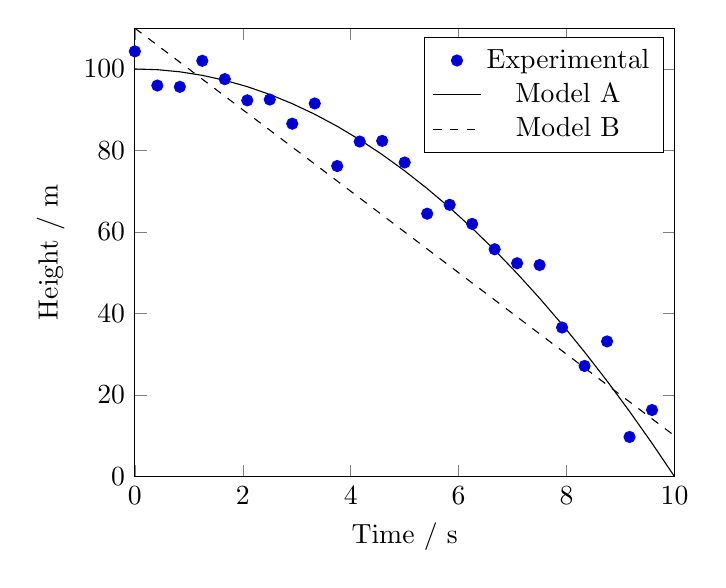
\begin{tikzpicture}
    \begin{axis}[xlabel=Time / s, 
                 ylabel=Height / m, 
%                 ylabel style={rotate=-90, anchor=east},
                 domain=0:10,
                 ymin=0,ymax=110,
                 enlargelimits=false]

      \addplot+[only marks] expression {100 - x^2 + rand*10};
      \addlegendentry{Experimental};
      \addplot[solid] expression {100 - x^2};
      \addplot[dashed] expression {110 - 10*x};
      \addlegendentry{Model A};
      \addlegendentry{Model B};
    \end{axis}
  \end{tikzpicture}
  \caption{Example of a figure.  Note that the line types are easy to
    distinguish without a colour display.  Include a citation in the caption if the figure is from referred source.}
  \label{fig:figexample}
\end{figure}

Use similar fonts (both size and lettertype) in the figure as in the
main text and always ensure that the caption explains the figure in
more detail than ``A plot of height over time''---this is visible from the
graph.

Figures containing photographs should be processed to be legible in
black and white, including labels.

\subsubsection*{Dos and don'ts}
\begin{itemize}
\item Do ensure that the fonts in your picture are clearly legible
\item Do use linetypes that are distinguishable in black and white reproductions
\item Do use suitable axes for showing the information you need to be seen (logarithmic for exponential behaviour, etc)
\item Do use suitable orders of fits if fitting.
\item Do include detail in the caption (about number of experiments, variance)
\item Do use the caption to tell the reader what to look for in the graph/picture.
\end{itemize}

\begin{itemize}
\item Don't fit splines (smooth curves) through all the data points 
\item Don't use ``computerisms'' like degC instead of \si{\celsius}\ or 1.2e2 instead of \num{1.2e2} 
\item Don't connect discrete experimental results with lines or connect data when there are not enough to suppose interpolation holds
\end{itemize}

\subsection{Tables}
Avoid lines in tables as much as possible (even on the sides
of tables---tables are not ``boxed in'').  The vertical
lines of figures should be enough to guide the eye vertically.  A
slightly thicker line should be used at the top and bottom of the
table, with a thin line between the headings and the data, as shown in
Table~\ref{tab:tabexample}.

\begin{table}[htbp]
  \centering
  \caption{Example of a table (adapted from \citet{fear})}
  \label{tab:tabexample}
  \begin{minipage}{0.5\textwidth}
    \begin{centering}
      \begin{tabular}{@{}llr@{}} \toprule 
        \multicolumn{2}{c}{Item}                                               \\ 
        \cmidrule(r){1-2} 
        Animal                    & Description & Price\textsuperscript{a} (R) \\ 
        \midrule 
        Gnat                      & per gram    & \num{13.65}                  \\ 
                                  & each        & \num{0.01}                   \\ 
        Parrot\textsuperscript{b} & stuffed     & \num{92.50}                  \\ 
        Emu                       & stuffed     & \num{33.33}                  \\ 
        Armadillo                 & frozen      & \num{8.99}                   \\ 
        \bottomrule 
      \end{tabular}                                                            \\
    \end{centering} 
    \vspace{1em}
    \textsuperscript{a} As of 2004                                             \\
    \textsuperscript{b} Norwegian blue only
  \end{minipage}
\end{table}

Units should be specified in the heading of a column and longer descriptions included as footnotes below the table.
Never split a figure or a table across two pages.
If more space is required than a single page, it is usually a sign that the material should be split into separate tables.
Always use a reasonable number of significant digits in your table.

\subsection{Cross-referencing}
When referring to items in the same text, use capitals and the
correct number as in the following example. 
Never state the number separately from the item name. 
Use ``Figure 1 and Figure 2'' instead of ``Figures 1 and 2''.

\begin{quote}
  As can be seen from Figure~1, Figure~2 and Figure~4, there is a strong
  correlation between heat transfer and Reynolds number.  Equation~2
  shows the proposed model, while Equation~3 has an alternate
  formulation proposed by Smee (1992).  The experimental results are
  summarised in Table~3.  Section~4 discusses these results in more
  detail, while Section~5 proposes novel research directions.
\end{quote}

\emph{Each and every sketch, figure and  table must be referred to in the text.} 
Place figures and tables as close as possible to their first reference (but definitely after the first reference).  


\subsection{Abbreviations}
\label{sec:abbreviations}
Our guidelines are adapted from \citet[17]{burger}.  All abbreviations
are written without periods or spaces (New Testament $\rightarrow$
NT).  Abbreviations are written as spoken. Capitals are used when the
single letters are pronounced (CSIR) while normal casing is sometimes used
when they are pronounced as a word (Unisa).  Always defer to the
preference of organisations regarding the spelling of their names
(SAIChE, ECSA).  Try not to use abbreviations unless they are in
common use.  If an abbreviation is not likely to be understood by the
audience, spell it out the first time and introduce the abbreviation
in parentheses: South African Institution of Chemical Engineers (SAIChE).

\subsection{Bullets}
\label{sec:bullets}
Bullets are very useful as informal counters (instead of 1, 2, 3 or a, b, c), but guard against bullet overuse.
Do not, for example, bullet every paragraph in a abstract or introduction.

\section{Structuring the Report/Paper}
\label{cha:structure}

\subsection{Title}
\label{sec:title}
The title is a short, \emph{informative} description of the
investigation.  It must be unambiguous and free of all unnecessary
words, but must contain the important keywords describing the
investigation. Many technical journals limit the title to 15 words.

\citet{mandersloot} offers the following advice:
\begin{itemize}
\item Avoid insignificant words and especially non-specific words like
  Investigation, Studies, Evaluating, Estimation, Method, Treatment,
  Assessment, Modelling, Application etc. In many instances the
  non-specific word can not be eliminated. In such cases do not start
  the title with these words---use them somewhere else in the title.

\item To maximise impact, start the title with the most significant
  issue---the Action or (more specific) the Subject of the action.
  For example: ``Optimisation for the design of dividing wall columns''
  is of interest to those who are considering using such a column,
  therefore it calls for a title: ``Dividing wall column optimisation''

\item Constrain the title to the main issues. For example ``Adding
  value to SA raw materials---selective synthesis of thymol from
  m-cresol over zeolite catalysts'' does not cover raw materials
  (plural) but one only. Mention this side issue in the text, but
  choose a title like ``Selective m-cresol conversion to thymol over
  zeolite catalysts'' or better ``M-cresol to thymol; selective
  conversion over zeolite catalysts''.  The semi-colon (or even the
  colon) is a very useful tool for turning titles around.
\end{itemize}

\subsection{Editorial information}

\subsubsection{Reports}
Figure~\ref{fig:reportformatsummary} shows a summary of the information that
will be found in a report.  Refer to Table~\ref{tab:format}.

\begin{figure}[htbp]
  \centering
  \fbox{
    \begin{demopage}
      \begin{centering}
        \vfill
        \textbf{Title of Report} \\
        \vfill
        {\small Student, A} \\
      \end{centering}
      \vfill
      \begin{flushright}
        \small CXX323 \\ \today
      \end{flushright}
    \end{demopage}
  }
  \fbox{
    \begin{demopage}
      \begin{centering}
        \textbf{Title of Report} \\
        \vfill
        {\small 
        Student, A \\
        20232329 \\
        Department of Chemical Engineering \\
        University of Pretoria }\\
        \vfill
        \begin{flushright}
          \small CXX323 \\ \today
        \end{flushright}
      \end{centering}
    \end{demopage}
    }
  \fbox{
    \begin{demopage}
      \centerline{\textbf{Title of Report}}
      \vspace{1em}
      \textbf{Abstract}\\
      {\small Scope, main findings, main conclusions. \\ }
      Keywords: a, b, c
      \vfill
%      \textbf{Sinopsis}\\
%      \rule{0.9\textwidth}{2pt} \\
%      \rule{0.9\textwidth}{2pt} \\
%      \vfill
      \begin{centering}
        ii \\
      \end{centering}
    \end{demopage}
  }
  \fbox{
    \begin{demopage}
      \textbf{Contents}\\
      {\small 
        Abstract\dotfill ii \\
        Nomenclature\dotfill iv \\
        1. Introduction\dotfill 1}
      \vfill
      \begin{centering}
        iii \\
      \end{centering}
    \end{demopage}
    }
  \fbox{
    \begin{demopage}
      \textbf{Nomenclature}\\
      {\small 
        $b$ Constant \hfill s \\
        $v$ Velocity \hfill km/h \\
        \\
        Greek\\
        $\alpha$ Force coefficient \hfill{1} \\
        $\rho$ Density \hfill kg/m\textsuperscript{3}}
      \vfill
      \begin{centering}iv\\ \end{centering}
    \end{demopage}
    }
  \fbox{
    \begin{demopage}
      \raggedright
      \textbf{1. Introduction}\\
      {\small Background, problem statement, purpose, method, scope \\
        (see~\ref{sec:introduction})
      }
      \vfill
      \begin{centering}1\\ \end{centering}
    \end{demopage}
  }
  \fbox{
    \begin{demopage}
      \textbf{2. Theory}\\
      {\small \begin{raggedright} Summary of the relevant theory, including ample
          references (see~\ref{sec:literature}) \\ \end{raggedright}}
      \vfill
      \begin{centering}2\\ \end{centering}
    \end{demopage}
    }
  \fbox{
    \begin{demopage}
      \textbf{3.~Experimental}\\
      {\small Apparatus, planning and methods \\ (see~\ref{sec:experimental})}
      \vfill
      \begin{centering}3\\ \end{centering}
    \end{demopage}
    }
  \fbox{
    \begin{demopage}
      \textbf{4. Results and Discussion}\\
      {\small \begin{raggedright} Supporting evidence, most important
          results first.  Use graphs and tables where
          possible. Explain the observed correlations
          between variables. (see~\ref{sec:results-and-discussion}) \\ \end{raggedright}}
      \vfill
      \begin{centering}4\\ \end{centering}
    \end{demopage}
    }
  \fbox{
    \begin{demopage}
      \raggedright
      \textbf{5. Conclusions and Recommendations}\\
      {\small Main findings  \\ No new information  (see~\ref{sec:conclusions-and-recommendations})}
      \vfill
      \begin{centering}6\\ \end{centering}
    \end{demopage}
    }
  \fbox{
    \begin{demopage}
      \raggedright
      \textbf{6. References}\\
      {\small Complete list of references in text.  Not a reading list (see~\ref{sec:references}) \\ }
      \vfill
      \begin{centering}8\\ \end{centering}
    \end{demopage}
    }
  \fbox{
    \begin{demopage}
      \textbf{A. First Appendix}\\
      {\small \begin{raggedright} Include only if necessary. Not a place to dump raw figures or calculations \\ \end{raggedright}}
      \vfill
      \begin{centering}9\\ \end{centering}
    \end{demopage}
    }

  \caption{Report format at a glance}
  \label{fig:reportformatsummary}
\end{figure}

The title of the report and the name(s) of the author(s) appear on the
\emph{cover}. This may be on specially textured paper or simply the
outermost page of the report.  Compare this to a published book.  In
the case of reports written for a specific university course (like CPY
311 or CLB 321) the course code and the hand-in date is displayed at
the bottom right hand corner of the cover.  Laboratory reports and
similar documents would normally not require a cover---the first page
is then the title page.

The first page is the title page on which the title and the author's
name again appear, as well as additional information like the name of
the institution, company or authority under whose name the report is
published and the date.  For university reports the student's number
and the course name and code will be given.  In the case of formal
academic dissertations and for some laboratory reports, the university
prescribes the format of the title page.  The information is arranged
intelligently to create a balanced impression.  The cover and title
page do not have visible numbering.

The \subsectionname{abstract} appears on the very next page, to enable
the cursory reader to find out immediately what the main findings and
recommendations (if any) are.  Because the abstract is always read
together with the title, the title is repeated.  If a translated
abstract is given and both do not fit on one page, the translated
abstract must start on a new page.
\subsectionname{Keywords} appear immediately after
the abstract.  See~Section~\ref{sec:abstract-keywords} for detailed
requirements regarding a abstract and keywords.

If the author wishes to thank persons or other instances, this is done
on the following page under the
heading \subsectionname{Acknowledgement(s)}.

The table of contents is given on the following page under the heading
\subsectionname{Contents}.  Each chapter or section is assigned a number and the number
of the page on which the chapter starts is shown.  The page on which
the introduction starts is page~number~1.  Use a decimal numbering
system for the headings of chapters, paragraphs and sub-paragraphs.
Avoid subdivisions with more than four digits (1.2.3.4.5).  Such
further divisions can be done in the text (but not shown in the table
of contents) with an alphabetical notation. The table of contents does
not include an item ``Contents''.

After the table of contents the nomenclature list is given (in
alphabetical order) under the heading \subsectionname{Nomenclature}.  All
symbols used are defined and the units are given.
The BIPM recommends that \href{https://www.bipm.org/en/publications/si-brochure/section5-3-7.html}{dimensionless quantities have dimensions of ``1''} (the
number one).
Greek
characters, subscripts and superscripts are tabulated separately.
This list is generally only required if several equations are employed
in the text.  The nomenclature list does not include abbreviations,
acronyms, chemical formulae, and so on.

The pages on which the editorial information (abstract, \dots nomenclature) appears are visibly numbered with small roman numerals (i, ii, \dots).
These pages are also indicated in the table of contents.  The
headings (abstract, contents, nomenclature etc) of the editorial
information are not numbered.

\subsubsection{Papers (Journal Articles)}
Figure~\ref{fig:paperformatsummary} shows a summary of information
that will be found in a paper. Refer to Table~\ref{tab:format}.
\begin{figure}[htbp]
  \centering
    \fbox{
    \begin{demopage}
      \begin{centering}
        \vfill
        \textbf{Title of Article} \\
        \vfill
        {\small Student, A and Lecturer, B \\ Department of Chemical
          Engineering \\ University of Pretoria \\
        \vfill
        {\small Abstract} \\
        \rule{0.9\textwidth}{2pt} \\
        \rule{0.9\textwidth}{2pt} \\
        \vfill
        Keywords: a, b, c
        }
      \end{centering}\\
      \vfill
    \end{demopage}
  }
  \fbox{
    \begin{demopage}
      \textbf{Nomenclature} \\
      \rule{0.9\textwidth}{2pt} \\
      \rule{0.9\textwidth}{2pt} \\
      
      \textbf{1. Introduction} \\
      \rule{0.9\textwidth}{2pt} \\
      \rule{0.9\textwidth}{2pt} \\
      \vfill
      \begin{centering}2 \\ \end{centering}
    \end{demopage}
  }
  \fbox{
    \begin{demopage}
      \rule{0.9\textwidth}{2pt} \\
      \rule{0.9\textwidth}{2pt} \\
      
      \textbf{5. References} \\
      \rule{0.9\textwidth}{2pt} \\
      \rule{0.9\textwidth}{2pt} \\
      \vfill
      \begin{centering}5 \\ \end{centering}
    \end{demopage}
  }

  \caption{Paper format at a glance}
  \label{fig:paperformatsummary}
\end{figure}

A paper does not have a cover.  The title page should contain the
following:
\begin{itemize}
\item The title in capitals, centred and not underlined.
\item Name/names of author(s), company affiliation(s) and address of
  the author to whom correspondence must be addressed.
\item A heading ``Abstract'', followed by the abstract of 100 to
  200 words.
\item A heading ``Keywords:'' at the left margin, followed (on the same
  line) by the keywords (generally no capitals).
\end{itemize}

Nothing else appears on the title page.  The information on the title
page is arranged to form a balanced layout, \emph{limited to one page only}.

The page numbers are counted from the title page using ordinary (Arabic) numerals.  
The title page number is usually not shown. 
The second page therefore is the first numbered page. 
It will show the number 2.  
If a nomenclature list is used, this appears at the top of page two, followed directly by the introduction.
If the headings are numbered, number 1 is assigned to the \subsectionname{Introduction}.  

The remaining sections proceed as for a report.  The theory section of
an article is usually more brief than in a report, as the readership
of the journal will typically be familiar with the subject matter.

\subsection{Abstract and keywords}
\label{sec:abstract-keywords}
The abstract is complementary to the title and is read together with
the title.  All the elements which appear in the title need therefore
not be repeated in the abstract.  The purpose of the abstract is to
summarise the
\begin{itemize}
\item scope of the investigation, if necessary
\item main findings and
\item main recommendations (if any).  
\end{itemize}
If the scope is not clear from the title, it can usually be defined
with a one sentence objective statement.  If the purpose of the
investigation is not clear from the title and the main findings, this
is also mentioned.  The abstract must, however, not contain phrases
like ``An investigation was launched~\dots'', ``\dots~is discussed'' or
``In this report/paper~\dots~is given/discussed/described~\dots''.

Important numerical information must be included in the abstract.  
If this is negelected, the abstract will have no impact.
Use paragraphs where appropriate.

Keywords are used in information retrieval systems.  
During a search of this nature papers with a certain keyword or combination of
keywords are selected.  
Choose a maximum of five words to characterise the report, and choose them carefully.  
Keywords should not be too general.

eg Keywords:   small letters, same line

\subsection{Introduction}
\label{sec:introduction}
The purpose of the introduction is to put the reader in the position
where the author was before he/she started the investigation.

The following usually appear in the introduction (but not as seperate sub-headings)
\begin{itemize}
\item Background
\item Problem statement
\item Purpose of the investigation (objective statement)
\item Method (very, very brief) and scope
\end{itemize}

In principle, only enough background should be given to enable the
reader to understand the problem statement.  The problem should be
stated in such a way that the objective can be understood.
It is always wise to state the objective statement in more detail than simply to solve the problem.

In general, the problem statement outlines the justification for the
investigation.  For example: 
``The problem is a shortage of potassium for the manufacture of fertilisers.'' 
The purpose of the investigation could then be to determine the feasibility of a filtration technique to purify a locally available raw material containing potassium.

The method and scope are mentioned only.  For that no
more than a few sentences will be required.  Further details can be
given in the body of the report.  For example: ``The efficiency is
determined experimentally in a laboratory scale investigation.
Because of compressed air limitations, the investigation is limited to
\SI{300}{\kilo\pascal}.''  or ``The number of swimming pools in the Pretoria
municipal area was determined from aerial photographs.  Indoor pools
are, therefore, not included.''  The scope statement is not a
list of excuses why some things were done badly or not at all. Neither is it a list of shortcomings in apparatus.

\subsection{Theory or literature}
\label{sec:literature}
A chapter on literature is included if more comprehensive background
is required than can conveniently be given in the introduction.  This
background will include information of which the reader is probably
not aware and which is required to understand the report, to justify
the investigation and to follow arguments and mathematical models or
expositions.  A review of \emph{relevant} literature \emph{must} be
given in all project reports, laboratory investigations and
dissertations.

It is totally undesirable to rewrite major portions of something like a
laboratory guide or textbooks, or to give detailed derivations of
equations.  Show only a summary of the current state of the art.
Referencing must be used to indicate the source of each statement or
data and each equation or derivation used in the literature chapter.

The literature section for a paper will of necessity be less
comprehensive than for a full report.  It should, however, always
convince the reader that the investigation method and the experimental
design were justified and that these were guided by the existing level
of knowledge on the subject.  The literature section should
not be a survey of all the literature published on the topic.  Only
the relevant literature should be discussed.  Never use the heading
Literature ``Survey'' for this section.

\subsection{Experimental}
\label{sec:experimental}
\subsubsection{Reports}

In reports the apparatus, planning and experimental methods are
described in some detail.  These can be included in one paragraph or
each can be assigned a separate paragraph.  The description and/or
references must be complete enough to enable the informed reader to
repeat the experimental work.

\paragraph{Materials List}
List the materials and chemicals used, their purities, and suppliers.

\paragraph{Apparatus} 
Describe the apparatus used.  Use sketches and give dimensions if
necessary.  Give equipment type and model number only if very specialised
equipment is used.  Do not present the apparatus as a ``shopping
list'', use full sentences. 

\paragraph{Analytical instruments}
List the make and model of all the analytical instruments used for your work. Do not use bullets for this.

\paragraph{Planning}
This is the experimental design.
Name the independent variables and justify the choice.  Justify the
range of values investigated for the independent variables used.  Show
and justify the choice of dependent (or measured) variables.  Show the
experimental design.  There are a number of good books on experimental
design, among others one by \citet{hicks}.  Note that
``experimental design'' is not the design or choice of equipment or
the experimental setup.  It concerns the variables in the experiment,
not the hardware.

\paragraph{Methods}
Without using an idiot recipe style, describe the methods used in the
experimental work and analysis.  Use references freely; also
references to standard methods and techniques such as methods of
chemical analysis.

\subsubsection{Papers}
The experimental section in a paper is as brief as possible, but it
must still be informative.  In many cases the three sections
(Apparatus, Planning and Methods) will be combined.  
Less detail will be given and referencing will be generous.

\textbf{Try not to reference the full report on which the paper is based}.

\subsection{Results and discussion}
\label{sec:results-and-discussion}
If it is immaterial to logic and flow of argument, report the most
important results first.  Use graphical and tabular presentation
judiciously, favouring graphical presentation.  Do not, in the same
report, show the same data graphically and in tabular form.  Indicate
important points to the reader.  
Report the results and immediately discuss their significance.

In reports, illustrate data manipulation using complete sample
calculations.  If it is feasible (for example in laboratory reports)
sample calculations are placed here, but mostly these are placed
separately in an appendix and referred to here.  In the case of large
projects, make meaningful subdivisions so that results do not
disappear in the variety of data, calculations etc.

\emph{Note:} Generally it is a good idea to subdivide the results and discussion section.
Sub-headings assist greatly in providing structure to a report or paper.

In papers, data manipulation and sample calculations are not generally
shown.  It may at times be necessary to tell the reader (in principle)
how the observed values were manipulated to arrive at the information
presented.

The results of most technical projects are in the form of correlations
between different variables.  The correlations must be explained using
accepted theories and mechanisms.  In the case of research projects,
new theories or mechanisms must be formulated.

The discussion and interpretation of your results will lead to
conclusions being drawn.  These conclusions should not merely be a
summary of results or observations, but rather show how these results
have been interpreted to form a new statement.
All conclusions must be based on results and reported in this section.

\subsection{Conclusions and Recommendation}
\label{sec:conclusions-and-recommendations}
This chapter is a summary of all the conclusions already drawn in the results and discussion chapter.
There will consequently be some repetition.
The most important conclusions must be mentioned first, unless this leads
to bad logic or loss of argument.  No new material, information or
conclusions may be introduced at this point.

All the objectives of the investigation, as stated in the
\subsectionname{Introduction}, must be addressed here.  
If this is not possible, the \subsectionname{Introduction} must be revised.
All conclusions mentioned here, must have been discussed beforehand.  
All conclusions must be based on results.

Findings may lead to actions which should be considered.  The
recommended actions are summarised as recommendations.  All
recommendations must be justified or justifiable from the conclusions.

\subsection{References}
\label{sec:references}
References should not be confused with headings like ``Bibliography''
or ``Further reading'', which frequently appear in non-technical
reports.  All references must be referred to in the text. Technical
reports and papers do not contain headings like ``Bibliography''.

Except for generally known facts, \emph{all statements that are
not your own must be provided with a reference}.  Never create the
impression that ideas, arguments, facts or conclusions are your own
unless this is true.  Plagiarism is a serious academic offense and may lead to disciplinary action, including up to two year's suspension.
Students are often unclear as to what constitutes plagiarism.  A good
rule of thumb is to reference \emph{everything} that you did not
create yourself, \emph{and} any statements that you may have thought
of yourself but may be controversial or counter-intuitive.  At an
undergraduate level it is unlikely that a student will come up with
something that has not been researched before.  If you have not found
supporting references, you have probably not looked hard enough.  For
more information, browse the University's plagiarism site at
\url{http://www.ais.up.ac.za/plagiarism}.

References are typically used to 
\begin{itemize}
\item justify statements and findings
\item enable the reader to consult the original source and
\item acknowledge the author(s) for a specific
  contribution~\citep{burger}.
\end{itemize}

The following statement need not be referenced: `` \dots at
the conclusion of the Second World War in 1945 \dots''

Consult the original source as far as possible, since it will usually
contain the most accurate account of the findings and limitations of a
certain study.  If, however, this is not possible (or if it is not
available) the original source can be cited as follows: ``Paul (quoted
in Strathmann, 1988) found that \dots''.  

Quotes from another person's work must clearly be shown as such, with
reference to the source.  Use ``quotation marks'' (Zeb, 1998) for
short quotes and paragraph indentation for longer ones:

\begin{quote}
  On two occasions I have been asked, `Pray, Mr Babbage, if you put
  into the machine wrong figures, will the right answers come out?' I
  am not able rightly to apprehend the kind of confusion of ideas that
  could provoke such a question. (Babbage, 1865)
\end{quote}

In our field of science, direct quotations
are seldom used; exceptions are possibly found in review articles or
in articles with a qualitative or speculative tendency.  When citing
indirectly, only the direct source (the one you read) is included in
the list of references.

See~Appendix~\ref{app:reference_methods} for a detailed discussion on
reference methods.

\subsection{Appendices}
\label{sec:appendices}
\subsubsection{Reports}
The previous chapters form the core of the report.  A good reporter
will arrange them to form a logical overview of the project.  To
achieve this it is usually necessary to exclude raw data, cumbersome
calculations, supporting results (for example standardising of
equipment) and documentary material (for example graphs used in
calculations and computer programs) from the main body of the
report.  Such material is then put in appendices as appropriate
paragraphs and subparagraphs.

Only one aspect is treated per appendix.  Each appendix is provided
with a number and descriptive heading and is indicated by page number
in the table of contents.  Every appendix must be mentioned in the
text.

Appendices should not contain unedited graphs, tables or figures.  The
symbols and language used in the appendices must be the same as in the
rest of the report.  If computer programmed results are used in
appendices, these must preferably be in the same letter type as the
rest of the report.  Printouts of things like statistical data must be
edited (or retyped) to eliminate unnecessary information and undefined
variables.

It is important to provide the reader with information about the items
in the appendix---explain why they were included and clear up some of
the more confusing aspects of the items.  An appendix is not a place
to ``dump'' information of only peripheral interest to the reader.

Appendices are letter-numbered starting at A. Refer to this document as an example.

\subsubsection{Papers}
Only in exceptional cases will a paper contain an appendix.  Such an
appendix should preferably not be more than one page and will not
necessarily start on a new page.

\section{Editing}
\label{cha:editing}
The process used for editing is used for marking of the student's
report or paper.  It forms the basis of the report editing checklist
given by \citet[176]{bruckmanmandersloot}.  This checklist is adapted
for use as a mark sheet in the Department.  It is the responsibility
of the author to scrutinise and grade his/her report in the same
manner (or to have it done) before it is submitted to the main reader.
A good author will wait a few days after writing the report before
doing this exercise.

Read the \strongemph{introduction} first.  Does it place the
investigation in context? Does it give background, problem
statement, purpose/aim, limitations and scope of the investigation?
See~Section~\ref{sec:introduction}.  Now read the
\strongemph{conclusions}.  Do the conclusions link directly with the
aims/purpose as set in the introduction?  Are the most important
conclusions offered first?  Is there a reason why not?  Are the
conclusions clear and unambiguous?  See
Section~\ref{sec:conclusions-and-recommendations}.

The reader should now have a good idea of the success of the
investigation.  Page through the report and look at the
\strongemph{headings}.  Is the hierarchy of headings correct?  Do
the numbers or letter type indicate the importance of the heading?  Is
it clear that all the important aspects are included?

Now the \strongemph{report} is read in its entirety, starting at the
introduction.  Note the content of each sentence and group of
sentences (text analysis) to ensure that the text appears in the
correct place in the report.  (A trained editor will already have done
text analysis on the introduction and conclusions at the first
reading).

After text analysis one may find that:
\begin{itemize}
\item there are results in the introduction
\item discussion is included in the part of the report that deals with
  experimental work
\item new experimental details are included in the results and discussion
\item discussion is included in the section that contains conclusions
\item some conclusions are not based on results
\item some recommendations do not flow from conclusions
\end{itemize}

Also take care to include the following issues:

Judge the author's use of the theory and literature chapter(s).  Is
there a critical analysis of the relevant literature and theory?  Are
the criteria used during the investigation properly identified?  Has a
decent experimental design been done?  See
Section~\ref{sec:experimental}.

Are results properly arrived at and presented?  Are graphical
presentations used efficiently?  Note the significance of data and the
correctness of sample calculations.  See~Section~\ref{sec:results-and-discussion}.
Gauge the author's insight from the discussion, the interpretation of
the results and significance of relationships and correlations.  Is
evaluation done using criteria that are identified in the literature?
Are valid conclusions drawn?  Has new material been introduced in the
conclusions?

The reader should now be well acquainted with the investigation and
can analyse the \strongemph{abstract} and the \strongemph{title}.  Are
the main findings, main recommendations and (if necessary) the purpose
and scope of the investigation clear from the abstract?  
Does the abstract have impact?
Do the title and abstract form a unit?  Is the title short and informative?  See
Section~\ref{sec:title} and Section~\ref{sec:abstract-keywords}.

Is the report prepared with the necessary editorial care?  Note
neatness, balanced page layout, care of language, spelling errors,
integrity with respect to numbering, grammatical parallelism of
headings and lists, sentence and paragraph construction, reference
technique and the correct application of conventions with regard to
figure and table titles.  A trained editor will have noticed most of these errors during the first reading of the report.

For verb tenses, consider the following:

\begin{quote}
    Use the past tense to report what happened in the past: what you did, what someone reported, what happened in an experiment, and so on. Use the present tense to express general truths, such as conclusions (drawn by you or by others) and atemporal facts (including information about what the paper does or covers). Reserve the future tense for perspectives: what you will do in the coming months or years. Typically, most of your sentences will be in the past tense, some will be in the present tense, and very few, if any, will be in the future tense \citep{doumont}.
\end{quote}

Does the report serve its \strongemph{purpose}?  Is the report
\strongemph{accurate}, \strongemph{brief} and \strongemph{clear}?  Is
the development logical?  Is the style acceptable?

It is strongly recommended that the report be read by a friend or
colleague for a final check on spelling errors and readability.

\newpage
\bibliography{techreport}
\bibliographystyle{chemeng}

%\appendix
\section{Appendices}
\appendix
\makeatletter
\def\@seccntformat#1{\csname Pref@#1\endcsname \csname the#1\endcsname\quad}
\def\Pref@section{Appendix~}
\makeatother

\section[Reference Methods: Policy of the Department of \\Chemical Engineering]{Reference methods: Policy of the \\Department of Chemical Engineering}
\label{app:reference_methods}
Two very popular reference methods are the Harvard method and the
augmented Harvard method.  Guidelines for the use of these methods are
contained in the International Standards Organisation (ISO) guideline
ISO 690 \citep{ISO690}.  \citet{burger} discusses these methods from
the perspective of a South African user.

In brief, the Harvard method quotes an author in the text by means of
a surname and the year of the publication, for example ``\dots was found.
(Smith, 1975)''.  The references are then given in alphabetical order
(according to the surname of the primary author) in the reference
list.  In the augmented Harvard method the text will contain a digit
which coincides with the position of the source in the reference list,
as in ``\dots was found.  [21]''.  The references are then given in
numerical order in the list of references.  Although the augmented
Harvard method is mostly used in scientific publications, we will, for
practical reasons, use the ordinary Harvard method in this department.

In practice a researcher/author will decide in which journal he/she
wishes to publish and will then adopt the reference style of that
journal.  Usually instructions/guidelines for authors appear at the
back of a journal, sometimes only in the December or January issue of
the journal.  Nevertheless, it is recommended that you scan the
journal for a paper with a decent list of references and use it as
your model.

It is recommended that you use an automated tool to generate your list of references, \textit{eg} EndNote, Zotero or Mendeley.

\subsection{References in the text}

In the general case the following are placed in parentheses at the point
of referencing in the text.

\paragraph{Books} Author's surname + comma + date of publication + colon +
page number like (Smith, 1988: 45) or (Smith \& Jones, 1999: 126).

\paragraph{Journals} Author's surname + comma + date of publication like
(Smith, 1988) or (Smith, Smith \& Jones, 2004).

Include initials if reference is made to more than one Smith like
(Smith, RP, 1988). Multiple references for the same fact are separated by semicolons 
(Miller, 1999; Shafranske \& Mahoney, 1998).

Special cases:
\begin{itemize}
\item If the date of publication is not known, use the copyright year
  or (if this not known): \emph{sa} [= \emph{sine anno}, no year], like (Smith,
  \emph{sa})
\item The page number is typically shown when reference is made to a
  certain place in the book and not when the whole book, an extract
  from a book or a journal article is referred to.
\item Two authors are linked with ``\&'' or ``and'' (Smith \& Klein, 1988).
\item For three or more authors, mention only the first followed by \emph{et al}.
  Thus Smith, Klein \& Long (1988) is written as Smith \emph{et al} (1988). Note that 
  there is no full stop, as described in Section \ref{sec:abbreviations}.  
  ``\emph{Et al}'' is short for \emph{et alii}, which means ``and others'' in Latin. 
  It is often translated as ``and coworkers'' when read in scientific context.
\item When the author is already mentioned in the text, the author's
  name is not repeated, like ``Smith (1988) found that \dots'' or
  ``Smith \& Jones (1999) found that \dots'' or ``Nicol \emph{et al} (2004)
  claim that \dots''
\item More than one reference for the same statement: (Smith \& Klein,
  1988; Peters, 1989) or ``Smith \& Klein (1988) and Peters
  (1989) found that \dots''.
\item Institutions must be referred to with minimum identification
  (Department of Energy Affairs, 1978) or (CSIR, 1987: 34).
\item If the same author published more than one publication in the
  same year, the publications are taken up alphabetically according to
  the title and marked ``a, b, c, \dots'', like (Smith, 1988a; Smith,
  1988b).
\item Secondary references, like when the original reference is not
  available, are treated as follows: (Smith, quoted by Peters, 1989:
  45).
\item Unusual author surnames: (Van der Merwe \& Day-Lewis, 1990).
\item Information taken from an encyclopaedia is treated in the same
  way as a chapter or section in an edited book.  The encyclopaedia
  article usually has an author who is cited in the text.  An example
  of a reference entry for this case is given in~\ref{sec:referencelist}
\end{itemize}

\subsection{A note on electronic documents}
With the common use of electronic resources and the Internet, it is
becoming more difficult to give a single reference for a physical
article.  There are several standards underway to provide a consistent
way of referring to on-line sources, but the URL (something like
\url{http://www.someaddress.com}) will not be connected with the same
information for any length of time.  For this reason, online sources
should be quoted only after exhaustive search for a physical reference
has yielded no results.  There are very few websites that exist
totally removed from any physical media---if you are referencing a
website for important information, there is a good chance they have
referenced their sources and you would do well to consult the original
material.

If there is no way to avoid citing a web reference, ensure that you
quote the date on which you visited the URL.

If you have obtained information from the documentation of a computer
program, cite them using the publishing company and a full version
number for the software (see the examples on
page~\pageref{page:ref_compsoftware}).  Remember to use an author and date
if this information is known.  As usual, refrain from using references
to computer media that may not be available to everyone---even if
``everyone'' is using the software now, it may not be available in
years to come.

\subsection{The reference list}
\label{sec:referencelist}

The cited references appear alphabetically in the reference list
according to the name of the first author.  Publications of the same
author are arranged chronologically and when author and year are the
same the sources are quoted alphabetically according to titles and
distinguished by alphabetical letters (like 1988a, 1988b).

All the authors are mentioned;  \emph{et al}  is never used in the
reference list.

Details of the publications are given in the following sequence:
author, year of publication and title; after that it depends on
whether the publication is a book, a journal or other work.  Most of
the options are indicated here as examples.  
Note that these groupings (Book, Paper, \emph{etc}) should not appear 
in the reference list.

Use headline capitalisation for the titles of books and journals (Fundamentals 
of Momentum, Heat and Mass Transfer; Journal of Fluorine Chemistry), but 
sentence capitalisation for the titles of papers, patents and reports 
(Influence of initiators on the sintering discolouration of PTFE).

\paragraph{Book}
The title of the book is in \emph{italics}. The page numbers of a book are not mentioned---they have already been given in-text. 

Kesting, RE (1972), \textit{Synthetic Polymeric Membranes}, 2nd edition,
  McGraw-Hill, New York.

Winkler, T, Botha, J, Kan, P and Rhodes, K (2006),
  \textit{Infinite Problems}, 1st edition, Wise Publications, Bloemfontein.

\paragraph{Paper published in a journal}
The title of the paper is in ``quotes'', while the journal name is in \emph{italics}. Give the volume number followed by the issue number in parentheses. Some journals indicate the issue or volume as a month and then the same rule applies. Write the page range with an en dash.

Strathmann, H (1981), ``Membrane separation processes''
  \textit{J  Membr  Sci}, 9(2), 121--189.

Adams, P and Adams, K (2006), ``The art of fermentation''
  \textit{Biotechnology Today}, 13(10), 22--30.

Jones, T, Stead, P and Krishner, V (1990) ``Filtration of salt
  on a rotary disc filter'' \textit{Filtration SA}, 36(6), 167--176.

\paragraph{Patent}
~

Henis, JMS and Tripodi, MK  (1980a), ``Multicomponent membranes
for gas separation'', \textit{US4230463A}, assigned to Monsanto
Corporation, USA.

Henis, JMS and Tripodi, MK (1980b), ``New method of producing
  defect-free membranes'', \textit{US4230454}, assigned to
  Monsanto Corporation, USA.

\paragraph{Report, thesis or similar}
Use italics and headline capitalisation for the title. Mention the type of 
report, \textit{eg} PhD Thesis, Master's Dissertation, or simply Technical Report.

Janzen, PA (1993), \textit{Clean Water Supply to Rural Communities},
  Zirkon Consultants' report to the Water Research Commission,
  Pretoria.
  
Van't Hof, J (1988), \textit{Wet Spinning of Asymmetric Hollow
    Fibre Membranes for Gas Separation}, PhD Thesis, University of
  Twente, Enschede.
  
O'Kelly, C (2001), \textit{Nanofiltration Membranes}, Project
  Report, Dept Chem Eng, University of Pretoria.

\paragraph{Encyclopaedia or similar}
If more than one editor (Ed) is mentioned, use the abbreviation (Eds).

Gmehling, J and Onken, U (1977--1980), ``Vapor-liquid
  equilibrium data collection'', Part 1 in \textit{Chemistry Data}, Part 7,
  Behrens, D and Eckermann, R (Eds), Dechema, Frankfurt am Main.

Peters, S (1991), ``Water soluble polymers'', in
  \textit{Ullmann's Encyclopedia of Industrial Chemistry}, A29, Wolff,
  R (Ed), VCR Vertrieb Publishers, D\"usseldorf.

Smolders, CA (1980), ``Morphology of skinned membranes: a
  rationale from phase separation phenomena'', in
  \textit{Ultrafiltration and Applications}, Cooper, I (Ed), Plenum
  Press, New York.

\paragraph{Reference in another publication}

Smith, SA quoted by Billiton, RS (1995), \dots followed by
  book, or journal reference.


\paragraph{Personal communication}
Never use personal communication references where a written reference
to the same information is available.  Never quote a lecturer on a
theoretical statement.  A reference should enable the reader to look
at your information.  Personal communications make this difficult.

Koros, WJ (1992), ``Glass transition properties of glassy
  polymers'', Personal Communication, Department of Chemical
  Engineering, The University of Texas at Austin.

\paragraph{Paper presented at a conference}
The year is shown between parentheses after the author(s) and often repeated when the conference dates are given.

Mazur, WH and Jakabhazy, SZ (1991), ``Gas separation 
  membranes---now 
  and tomorrow'', paper presented at \textit{The Europe-Japan
  Congress on Membranes and Membrane Processes}, 23--25 May, 1991,
  Stresa, Italy.

\paragraph{Web page}
The date in the square brackets is the access date.

Pritzker, TJ (1999), ``An early fragment from Nepal'',
  \url{http://www.ingress.com} [2000-06-08].  

\paragraph{Computer Software}
\label{page:ref_compsoftware}
~

Microsoft (2007), ``Add picture bullets or symbols to lists'',
  Microsoft Word 2007 help.

Stallman, R and MacKenzie, D (2007), ``LS(1) man page'', GNU
  coreutils v6.9, \url{http://www.gnu.org/software/coreutils/} [2019-01-01].
  
\paragraph{eBook}
Similar to a book but with a URL and access date. Give the version, publisher and city if mentioned. 

H\"unniger, D (2012), \textit{LaTeX Wikibook} 
  \url{https://upload.wikimedia.org/wikipedia/commons/2/2d/LaTeX.pdf} [2019-04-12].
 
Oetiker, T, Partl, H, Hyna, I, and Schlegl, E (2018), The Not So 
 Short Introduction to LaTeX 2$\epsilon$, Version 6.3,  \url{https://tobi.oetiker.ch/lshort/lshort.pdf} [2019-04-12].



Note: References to electronic media should be devised as author,
date, title as shown in the examples above. If a person cannot be 
named, use a corporate author such as ``Microsoft''. Include a DOI (digital object identifier) at the end if possible.

\subsubsection*{Important notes}

\begin{itemize}
\item The references are not numbered.  Paragraph spacing is used
  between references.
\item An author's initials are separated from the surname by a comma,
  following the abbreviation rules in Section~\ref{sec:abbreviations}.
\item When more than one author is mentioned, use ``and'' instead of an 
  ampersand (note that an ``\&'' may still be used in-text but be consistent).
\item Hyphenated surnames may not be shortened: Girard-Perregaux, AS (2012) \dots. 
  Give all initials for hyphenated names: Lin, Y-D (2008) \dots.
\item The patents of Henis \& Tripodi above have the same year and are arranged
  alphabetically according to the patent title.  If the second author had been
  different, the patents would have been arranged according to the
  second author.
\end{itemize}

It must again be emphasised that these guidelines hold for this
Department and that a number of alternative referencing systems are in
use.  A practical advantage of the Harvard method is that the
elimination and addition of references is done without it being
necessary to renumber all the references.  It is also often easier for
the reader if the referenced author is mentioned by name in the text,
instead of being identified as a number only.

\end{document}
